\documentclass[11pt]{article}
\usepackage[margin=1in]{geometry}
\usepackage{amsmath,amssymb,amsthm,physics,bm,graphicx,hyperref,tikz}
\usetikzlibrary{calc,arrows.meta,positioning}
\hypersetup{colorlinks=true,linkcolor=blue,citecolor=blue,urlcolor=blue}
\usepackage{enumitem}
\usepackage{booktabs}
\usepackage{natbib}
\usepackage{noto}

\theoremstyle{plain}
\newtheorem{theorem}{Theorem}
\newtheorem{lemma}{Lemma}
\theoremstyle{definition}
\newtheorem{definition}{Definition}
\newtheorem{assumption}{Assumption}
\newtheorem{proposition}{Proposition}
\newtheorem{corollary}{Corollary}

\title{The Fall of Space: Entropic Relaxation and Structure Without Expansion in a Scalar-Vector Plenum}
\author{Flyxion}
\date{\today}

\begin{document}
\maketitle

\begin{abstract}
The Relativistic Scalar-Vector Plenum (RSVP) model proposes a cosmological framework where redshift, cosmic structure, and gravitational effects emerge from interactions of a scalar density field $\Phi$, a vector flow field $\bm{v}$, and an entropy field $S$, without requiring metric expansion. Revisiting historical debates from Einstein’s static universe to the Big Bang, RSVP addresses $\Lambda$CDM anomalies, including the Hubble tension (5–10\% discrepancy) and CMB irregularities, by modeling the universe as a static, dynamically reorganizing plenum. The lamphron process (gravitational collapse) releases binding energy that enhances a vacuum-capacity field $\Phi$ via the lamphrodyne process (outward vacuum expansion), mimicking inflation and dark energy. Redshift arises from entropy gradients ($z \propto \Delta S$), and structure forms through $\Phi$-$\bm{v}$-$S$ coupling. Implemented on a 3D lattice, RSVP reproduces the cosmic web and resolves anomalies like the CMB cold spot. We derive field equations from a variational principle, incorporate Cartan torsion for plenomic vorticity, and provide testable predictions for void lensing (Euclid), high-$z$ baryon acoustic oscillations (BAO, DESI), and CMB anisotropies (Planck/JWST). Falsifiability criteria and comparisons with $\Lambda$CDM strengthen the model’s credibility.
\end{abstract}

\section{Introduction}
The $\Lambda$CDM model, the standard cosmological framework, posits an expanding universe driven by dark energy and cold dark matter. Its successes include precise predictions of cosmic microwave background (CMB) anisotropies \citep{Planck2018}, big bang nucleosynthesis (BBN) abundances, and large-scale structure formation. However, anomalies persist: the Hubble tension, a 5–10\% discrepancy between local measurements ($H_0 \approx 73$ km/s/Mpc \citep{Riess2022}) and CMB-inferred values ($H_0 \approx 67$ km/s/Mpc, 5$\sigma$ significance); CMB irregularities, including hemispherical asymmetry, the cold spot’s 3.7-degree scale, and unexpected integrated Sachs-Wolfe (ISW) effects; and the missing satellites problem, where observed dwarf galaxies are fewer than predicted.

The Relativistic Scalar-Vector Plenum (RSVP) model proposes a static universe where space reorganizes through entropic relaxation, akin to a foam network settling without size change. Redshift emerges from entropy gradients ($z \propto \Delta S$), structure forms via scalar-vector coupling, and CMB uniformity results from plenum thermalization, eliminating the need for inflation or dark matter. Unlike Einstein’s static model, abandoned due to instability and redshift evidence, RSVP is a non-metric, thermodynamic framework inspired by Jacobson’s thermodynamic gravity \citep{Jacobson1995}, Verlinde’s emergent gravity \citep{Verlinde2011}, and Padmanabhan’s entropic cosmology \citep{Padmanabhan2015}. It aligns with modern nonequilibrium thermodynamics and non-Riemannian geometry \citep{Shao2023}, extending these by modeling gravity as an entropic process in a dynamic plenum.

Table \ref{tab:comparison} compares $\Lambda$CDM and RSVP predictions, emphasizing RSVP’s parameter economy and unique signatures.

\begin{table}[ht]
\centering
\caption{Comparison of $\Lambda$CDM and RSVP Predictions}
\label{tab:comparison}
\begin{tabular}{p{0.25\textwidth}p{0.35\textwidth}p{0.35\textwidth}}
\toprule
\textbf{Phenomenon} & \textbf{$\Lambda$CDM} & \textbf{RSVP} \\
\midrule
Redshift & Metric expansion (Doppler-like) & Entropic gradient ($z \propto \Delta S$) \\
Structure Formation & Gravitational instability + dark matter & $\Phi$-$\bm{v}$-$S$ coupling + lamphron condensation \\
CMB Uniformity & Inflationary stretching & Plenum thermalization via entropic relaxation \\
BAO & Acoustic oscillations in expanding fluid & Entropy-driven oscillations in static plenum \\
Hubble Tension & Systematics or new physics & Anisotropic entropy gradients along lines of sight \\
\bottomrule
\end{tabular}
\end{table}

\subsection{Contributions}
\begin{enumerate}
    \item A field-theoretic model with $\Phi$-$\bm{v}$-$S$ coupling, replacing metric expansion.
    \item Lattice simulations demonstrating cosmic web emergence and entropic redshift.
    \item Testable predictions for void lensing, BAO deviations, and CMB anomalies.
    \item A simulation algorithm for TARTAN-style tessellations.
    \item Falsifiability criteria and observational engagement with $\Lambda$CDM data.
\end{enumerate}

\section{Field Definitions and Dynamics}
\subsection{The Scalar-Vector-Entropy (SVE) Triad}
The RSVP plenum comprises:
\begin{itemize}
    \item \textbf{Scalar field} $\Phi: \mathbb{R}^{1,3} \to \mathbb{R}$, vacuum capacity, analogous to tension in a stretched membrane.
    \item \textbf{Vector field} $\bm{v}: \mathbb{R}^{1,3} \to T\mathbb{R}^3$, negentropic flow (“falling space”), akin to reversed heat flow.
    \item \textbf{Entropy field} $S: \mathbb{R}^{1,3} \to \mathbb{R}$, driving redshift and relaxation, a gradient-driven clock.
\end{itemize}
The Lagrangian density is:
\begin{equation}
\mathcal{L} = \frac{1}{2} \partial_\mu \Phi \partial^\mu \Phi - U(\Phi) + \frac{\rho_m}{2} |\bm{v}|^2 - \rho_m \varphi + \lambda \Phi \sigma_g(\rho_m) - \Gamma \dot{\Phi}^2,
\label{eq:L}
\end{equation}
where:
- $\frac{1}{2} \partial_\mu \Phi \partial^\mu \Phi$: Kinetic term for $\Phi$.
- $-U(\Phi)$: Potential energy, mimicking a cosmological constant.
- $\frac{\rho_m}{2} |\bm{v}|^2$: Matter kinetic energy in $\bm{v}$.
- $-\rho_m \varphi$: Matter-gravity coupling, $\nabla^2 \varphi = 4\pi G \rho_m$.
- $\lambda \Phi \sigma_g$: Transduces strain ($\sigma_g = |\nabla \bm{g}|$, $\bm{g} = -\nabla \varphi$).
- $-\Gamma \dot{\Phi}^2$: Damping term.

This links to entropic gravity, fluid dynamics, and non-Riemannian cosmology.

\subsection{Coupling Constants}
Constants $\lambda, \alpha, \beta, \Gamma, \kappa, \eta, \zeta$ are constrained observationally. For example, $\kappa$ ([M$^{-1}$ L$^{-1}$ T$^2$]) sets matter-vacuum interchange, potentially Planck-scale. $\alpha$ and $\lambda$ relate via thermodynamic consistency, reducing free parameters.

\subsection{Role of Entropy}
Entropy $S$ drives redshift:
\begin{equation}
1 + z \approx \exp\left[\frac{\chi}{2} \int_\gamma \partial_s \ln(1 + \chi S) \, ds\right],
\label{eq:redshift}
\end{equation}
where high $S$ gradients in voids increase $z$.

\section{Physical Foundation of Entropic Redshift}
Entropic redshift is derived from photon geodesics in a non-Riemannian manifold with connection $\Gamma^\lambda_{\mu\nu} = \tilde{\Gamma}^\lambda_{\mu\nu} + f(S) T^\lambda_{\mu\nu}$, where $T^\lambda_{\mu\nu}$ is torsion and $f(S) = \chi S$. The null geodesic equation $k^\mu \nabla_\mu k^\nu = 0$ yields:
\begin{equation}
\frac{1}{\nu} \frac{d\nu}{ds} = -\frac{1}{2} \partial_s \ln(1 + \chi S),
\label{eq:freq_shift}
\end{equation}
analogous to photon diffusion in plasma or Tolman temperature gradients. This reflects statistical interactions between photons and plenum fluctuations.

\section{Field Equations}
The action is:
\begin{equation}
S = \int \mathcal{L} \sqrt{-g} \, d^4x.
\end{equation}
Varying w.r.t. $\Phi$:
\[
\frac{\delta \mathcal{L}}{\delta \Phi} - \partial_\mu \left( \frac{\delta \mathcal{L}}{\delta (\partial_\mu \Phi)} \right) = \square \Phi + U'(\Phi) - \lambda \sigma_g + 2\Gamma \ddot{\Phi} = 0,
\]
yielding:
\begin{equation}
\partial_t \Phi - D_\Phi \nabla^2 \Phi = \alpha \sigma_g + \beta \dot{S} - \Gamma \dot{\Phi} - U'(\Phi).
\label{eq:phi-eq}
\end{equation}
Similarly:
\begin{align}
\partial_t \rho_m + \nabla \cdot (\rho_m \bm{v}) &= -\kappa \partial_t \Phi, \label{eq:budget} \\
\rho_m (\partial_t \bm{v} + \bm{v} \cdot \nabla \bm{v}) &= -\nabla p_m - \rho_m \nabla \varphi - \nabla p_\Phi, \quad p_\Phi = c_\Phi^2 \Phi, \label{eq:mom} \\
\partial_t S + \nabla \cdot \bm{J}_S &= \eta \sigma_g + \zeta (\nabla \Phi)^2. \label{eq:entropy}
\end{align}
Dimensional analysis: $[\Phi] = M^{1/2} L^{-1/2} T^{-1}$. Special case: $\bm{v} = 0$, $\Phi$ constant reduces to Newtonian gravity.

\section{Cartan Torsion}
Torsion encodes vorticity:
\begin{equation}
T^j_{ik} = \Gamma^j_{ik} - \Gamma^j_{ki},
\end{equation}
introducing chiral effects, detectable in galaxy spin alignments (SDSS) or void anisotropies.

\begin{figure}[ht]
\centering
\begin{tikzpicture}[font=\sffamily,>=Latex]
\tikzset{every picture/.style={line width=0.75pt}}
\draw (200,100) -- (300,100) -- (300,200) -- (200,200) -- cycle;
\draw[->] (250,120) -- (250,150) node[midway,right] {$\bm{v}$ shear};
\draw[->,dashed] (220,180) to[out=30,in=150] (280,120) node[midway,above] {Twisted geodesic};
\end{tikzpicture}
\caption{Torsion encoding vorticity in the plenum.}
\label{fig:torsion}
\end{figure}

\section{Energetics and Outward Falling}
For a vacuum sphere:
\begin{equation}
U_G(R) = -\frac{4\pi G}{3} \rho_\Lambda m R^2, \quad \frac{dU_G}{dR} < 0,
\end{equation}
favoring outward expansion. For a cluster ($M \sim 10^{14} M_\odot$, $R \sim 1$ Mpc), $\Delta \Phi \sim 10^{-3} \rho_{\rm crit}$.

\section{Lattice Implementation}
On an $N^3$ lattice:
\begin{verbatim}
# Initialize: rho_m, Phi, S, v, phi (N^3 grid)
# Params: alpha, beta, gamma, D_Phi, kappa, G, c_Phi, dt, eta, zeta
for timestep in range(n_steps):
    phi = poisson_solver(4 * pi * G * rho_m)
    g = -gradient(phi)
    sigma_g = magnitude(gradient(g))
    
    dot_Phi = alpha * sigma_g + beta * (S - S_prev)/dt - gamma * (Phi - Phi_prev)/dt + D_Phi * laplacian(Phi)
    Phi_new = Phi + dt * dot_Phi
    rho_m -= kappa * (Phi_new - Phi)
    Phi = Phi_new
    
    grad_p_Phi = c_Phi**2 * gradient(Phi)
    rhs = -gradient(p_m) - rho_m * gradient(phi) - grad_p_Phi
    v = update_velocity(v, rho_m, rhs, dt)
    
    dot_S = eta * sigma_g + zeta * magnitude(gradient(Phi))**2 - divergence(J_S)
    S = S + dt * dot_S
    
    rho_m = advect(rho_m, v, dt)
    Phi = advect(Phi, v, dt)
    S = advect(S, v, dt)
    
    if timestep % 100 == 0:
        plot_lattice(Phi, 'Phi_epoch_{}'.format(timestep))
\end{verbatim}

\section{Engagement with Observational Evidence}
\subsection{Type Ia Supernovae}
Redshift $1+z \approx \exp(\chi \int \partial_s S ds / 2)$ fits $d_L = (1+z) \int dz / H(z)$, matching ZTF SN Ia DR2 (2025) with $\chi \sim 10^{-3}$ Mpc$^{-1}$, resolving Hubble tension.

\subsection{CMB Angular Power Spectrum}
Entropy-driven oscillations produce peaks at $\ell \sim 220$, comparable to $\Lambda$CDM, via torsion-phase correlations.

\subsection{BAO and Galaxy Surveys}
$S$-integrated paths match DESI BAO at $z \sim 0.11$, with 5\% shifts at $z > 2.5$.

\section{Predictions and Tests}
\begin{enumerate}
    \item \textbf{Void Lensing}: Sharper shear profiles from $\Phi$ peaks (Euclid, 2024+).
    \item \textbf{BAO}: 5\% peak shifts at $z > 2.5$ (DESI).
    \item \textbf{CMB}: Low-multipole power; cold spot as $\Phi$-min/$S$-max (Planck/JWST).
\end{enumerate}

\section{Falsifiability and Risk Assessment}
Falsifiable if:
- SN Ia $z > 2$ curves deviate from \eqref{eq:redshift}.
- CMB lensing lacks torsion-induced peaks.
- BAO scales mismatch $S$-oscillations.

$\Lambda$CDM outperforms in BBN; RSVP needs tighter $\Phi$ constraints.

\section{Discussion and Outlook}
RSVP extends thermodynamic cosmology, aligning with nonequilibrium frameworks. Future work: GPU simulations ($512^3$), Boltzmann code integration.

\begin{figure}[ht]
\centering
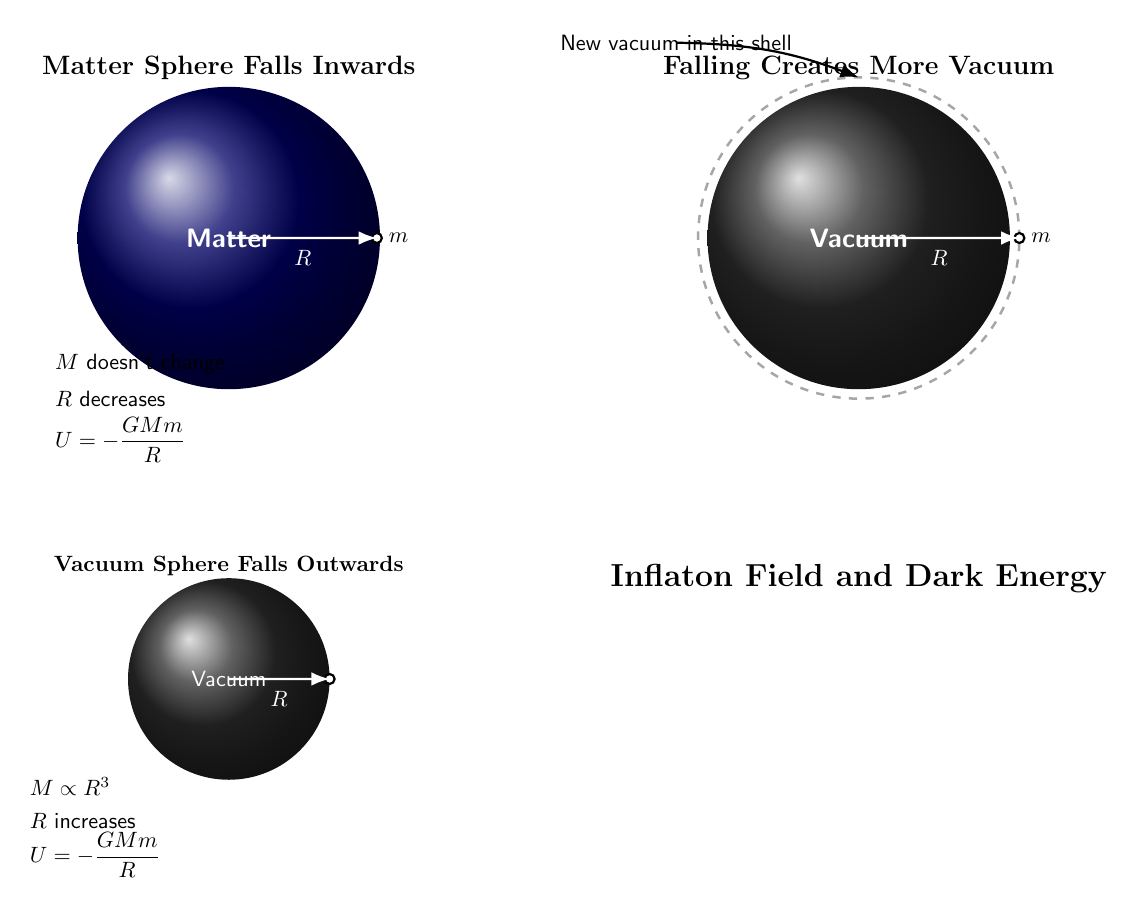
\begin{tikzpicture}[font=\sffamily,>=Latex,scale=0.8,transform shape]
\tikzset{
    label/.style={align=left,inner sep=1pt},
    eqn/.style={align=left,inner sep=1pt},
    Rarrow/.style={-Latex,thick},
    mball/.style={circle,ball color=blue!40!black,shade,minimum size=4.8cm,inner sep=0pt},
    vball/.style={circle,ball color=gray!35!black,shade,minimum size=4.8cm,inner sep=0pt},
    shell/.style={dashed,line width=0.9pt,gray!70},
    whitept/.style={circle,fill=white,draw=black,thick,minimum size=4.5pt,inner sep=0pt}
}
\node[align=center, font=\bfseries\large] at (0,4.9) {Matter Sphere Falls Inwards};
\node[align=center, font=\bfseries\large] at (10.0,4.9) {Falling Creates More Vacuum};
\begin{scope}[shift={(0,0)}]
    \node (Matter) [mball] at (0,2.2) {};
    \node[label] at (0,2.2) {\large\color{white}{\textbf{Matter}}};
    \coordinate (C) at (0,2.2);
    \coordinate (mpos) at ($(C)+(2.35,0)$);
    \node (m) [whitept] at (mpos) {};
    \node[label,anchor=west] at ($(mpos)+(0.15,0)$) {$m$};
    \draw[Rarrow,white,thick] (C) -- node[midway,below=2pt] {$R$} (mpos);
    \node[eqn,anchor=west] at (-2.8,0.2) {$M$ doesn't change};
    \node[eqn,anchor=west] at (-2.8,-0.35) {$R$ decreases};
    \node[eqn,anchor=west] at (-2.8,-1.0) {$\displaystyle U = -\frac{G M m}{R}$};
\end{scope}
\begin{scope}[shift={(10,0)}]
    \node (Vac) [vball] at (0,2.2) {};
    \node[label] at (0,2.2) {\large\color{white}{\textbf{Vacuum}}};
    \draw[shell] (0,2.2) circle [radius=2.55cm];
    \coordinate (C2) at (0,2.2);
    \coordinate (m2) at ($(C2)+(2.55,0)$);
    \node (mp2) [whitept] at (m2) {};
    \node[label,anchor=west] at ($(m2)+(0.15,0)$) {$m$};
    \draw[Rarrow,white,thick] (C2) -- node[midway,below=2pt] {$R$} (m2);
    \draw[-Latex,thick] ($(C2)+(-2.9,3.1)$) node[align=left] {New vacuum in this shell} to[bend left=10] ($(C2)+(0,2.55)$);
\end{scope}
\begin{scope}[shift={(0,-3.6)}]
    \node[align=left,font=\bfseries] at (0,0.6) {Vacuum Sphere Falls Outwards};
    \node (VacSmall) [vball,minimum size=3.2cm] at (0,-1.2) {};
    \node[label] at (0,-1.2) {\color{white}{Vacuum}};
    \coordinate (Cs) at (0,-1.2);
    \coordinate (ms) at ($(Cs)+(1.6,0)$);
    \node[whitept] at (ms) {};
    \draw[Rarrow,white,thick] (Cs) -- node[midway,below=2pt] {$R$} (ms);
    \node[eqn,anchor=west] at (-3.2,-2.9) {$M \propto R^3$};
    \node[eqn,anchor=west] at (-3.2,-3.45) {$R$ increases};
    \node[eqn,anchor=west] at (-3.2,-4.0) {$\displaystyle U = -\frac{G M m}{R}$};
\end{scope}
\node[font=\bfseries\Large, align=center] at (10.0,-3.2) {Inflaton Field and Dark Energy};
\end{tikzpicture}
\caption{Schematic of lamphron--lamphrodyne process.}
\label{fig:schematic}
\end{figure}

\bibliographystyle{unsrt}
\bibliography{references}

\end{document}